\chapter{Математические модели синтеза топологии сети для охвата линейного участка в виде задачи целлочисленного линейного программирования}\label{chapter_ilp_model}

% \section{Introduction}
% Wireless technologies are widely used in various areas of human life. Wireless broadband communication networks are used for operational control of industrial or civil objects, technological plants, smart moving vehicles. The use of wireless broadband technologies based on the IEEE 802.11 protocols family to organize such networks has several advantages over wired technologies. These include rapid deployment of communication networks, convenient modernization and scalability of the network architecture, and reduced installation and maintenance costs.

% To improve the design efficiency of such a modern information transmission infrastructure, it is crucial to solving the problem of optimal placement of equipment, in our case, base stations of a wireless broadband communication network at various possible locations. A similar problem has been proposed and discussed in several works \cite{KHireddine2020,BenBrahim2014,Chattopadhyay2018,KIZILOZ2020,Liu2014,Reis2014,Shen2020}.

% This work is a continuation of the researches \cite{Ivanov2018} and \cite{Ivanov2019}, where the particular case of the problem is considered when the controlled area is a linear section, for example, the area along highways, the linear part of trunk pipelines, field communications. In the above papers, the formulation was given in the form of an integer linear programming model. The proof of NP -- completeness was presented.

% The problem considered in the previous work \cite{Ivanov2019} it was necessary to place a given base station set formed at the previous network design stages. The present paper considers a more general case when solving an optimization problem is also determined by a set of placed stations from a given redundant set while respecting technical and economic constraints. This paper presents the preparation of main station characteristics, such as the coverage radius, link distance, and station service time. We need to prepare these characteristics before proceeding to the optimal placement problem.  The paper proposes the problem in the form of an integer linear programming with the input of the above-calculated characteristics into the problem conditions with the end-to-end delay constraint. This restriction significantly impacts the mathematical model form of the problem.


\section{Постановка задачи}

Проблема формулируется следующим образом. Для контроля над заданным линейным участком необходимо разместить базовые приемопередающие станции (далее называемые станциями) таким образом, чтобы максимизировать покрытие с ограничениями на суммарнуб стоимость размещенных станций. Важно обеспечить связи любой станции со шлюзами на концах участка через систему размещенных станций.

Задано множество станций $S = \{s_j\}$. Каждой станции приписаны параметры $s_j = \{r_j, \{R_{jq}\}, c_j \}$, $j = \overline{1,m}; q = \overline{1,m}; q \neq j$. Здесь $r_j$ -- радиус покрытия станции, $R_{jq}$ -- это радиус связи между станцями $s_j$ и $s_q$, и $c_j$ -- это стоимость. 

Задан линейный участок длиной $L$ с концами в точка $a_0$ и $a_{n+1}$. Внутри  отрезка $[a_0, a_{n+1}]$ задано конечное множество точек $A=\{a_i\}, i=\overline{1,n}$; эти точки соответствуют набору свободных мест, где могут быть размещены станции. Каждая точка $a_i$ определяется своей одномерной координатой $l_i$.

Заданы станции специального вида $s_{m+1}$ -- шлюзы. Данные шлюзы размещены на концах $a_0$ и $a_{n+1}$ данного линейного участка . Для данных станций параметр радиуса покрытия $r_{m+1}=0$. Радиус связи и стоимость не заданы.

Требуется разместить станции таким образом, чтобы максимизировать покрытие с условием ограничения на суммарное стоиомсть $C$.

 

% \section{Расчет дальности действия связи}


% Перед тем как приступить к задаче ЦЛП необходимо рассчитать характеристики станции: радиус связи $R_{jq}$ и радиус покрытия $r_j$.

% При развертывания сети необходимо обеспечить максимальное покрытие данного участка связь между шлюзами через систему размещенных базовых станций беспроводной широкополосной сети.

% Для оценки производительности канала связи воспользуемся уравнением энергетического потенциала. Полное уравнение можно записать следующим образом:

% % It is essential during deployment to provide maximum coverage of a given area and ensure communication between the placed base stations in the wireless broadband network. 

% % Link Budget is a way of estimation of communication link's performance while accounting for the system's power, gains, and losses for both the transmitter and receiver. The complete equation can be written as follows:

% \begin{equation}
%   \label{eq:part3_link_budget}
%   P_{tr} - L_{tr} + G_{tr} - L_{fs} + G_{recv} - L_{recv} = SOM + P_{recv},
% \end{equation}
% где:

% \begin{itemize}

%   \item $P_{tr}$ -- мощность передатчика, дБм;

%   \item $L_{tr}$ -- потери сигнала на антенном кабеле и разъемах передающего тракта, дБ;

%   \item $G_{tr}$ -- усиление антенны передатчика, дБ;

%   \item $L_{fs}$ -- потери в свободном пространстве, дБ;

%   \item $G_{recv}$ -- усиление антенны приемника, дБ;

%   \item $L_{recv}$ -- потери сигнала на антенном кабеле и разъемах приемного тракта, дБ;

%   \item $SOM$ -- запас на замирание сигнала, дБ;

%   \item $P_{recv}$ -- чувствительность приемника, дБм.

% \end{itemize}

% Мощность принимаемой антенны рассчитывается из уравнения передачи Фрииса:

% \begin{displaymath}
%   \label{eq:part3_Friis}
%   \frac{P_{recv}}{P_{tr}} = G_{tr}G_{recv}\left(\frac{c}{4\pi R f} \right)^2,
% \end{displaymath}
% где
% $c$ --  скорость света,
% $f$ -- частота, 
% $R$ рассточние между приемной и передающей антенной.

% The Free Space Path Loss ($ FSPL $) equation defines the propagation signal loss between two antennas through free space (air):

% Уравнение потерь в свободном пространстве (Free Space Path Loss, $FSPL $) определяет потерю сигнала при распространении между двумя антеннами в свободном пространстве (в воздухе):

% \begin{equation}
%   \label{eq:part3_FSPL}
%   FSPL = \left(\frac{4\pi R f}{c} \right)^2.
% \end{equation}

% Формула (\cref{eq:part3_FSPL}), выраженная в децибеллах будет выражаться как

% \begin{equation}
%   \label{eq:part3_L_fs}
%   L_{fs} = 20 \lg{F} + 20\lg{R} + K,
%   \end{equation}
% где $F$ -- центральная частота, на котором работает канал связи, $R$ -- рассточние между приемной и передающей антенной и $K$ -- константа.

% Константа $K$ зависит от размерностей частоты и расстояния:

% \begin{itemize}
%   \item для чистоты, выраженной в ГГц, и рассчтояния, выраженная в км, константа $K$ равна 92.45;
%   \item для чистоты, выраженной в МГц, и рассчтояния, выраженная в км, константа $K$ равна 32.4;
%   \item для чистоты, выраженной в МГц, и рассчтояния, выраженная в м, константа $K$ равна -27.55.
% \end{itemize} 

% Потерия $L_{fs}$ выразим из формулы (\cref{eq:part3_link_budget}) как:

% \begin{equation}
%   \label{eq:part3_L_fs_from_link_budget}
%   L_{fs} = P_{tr} - L_{tr} + G_{tr} + G_{recv} - L_{recv} - SOM - P_{recv}.
% \end{equation}

% Радиус связи получаем из уравнений (\cref{eq:part3_L_fs}) и (\cref{eq:part3_L_fs_from_link_budget}):

% \begin{equation}
%   \label{eq:part3_D}
%   R = 10^{\left(\frac{L_{fs} - 20\lg{F} - K}{20}\right)}.
% \end{equation}

% Используя формулу \cref{eq:part3_D} и \cref{eq:part3_L_fs_from_link_budget}, мы можем расчитать теоритическое максимальную дальность связи $ R_{jq}$ между базовыми станциями и радиусом покрытия $ r_j $ с предположением об отсутствии препятствий, отражений, влияния контуров местности и т. д. Это допущение приемлемо для нашего случая с открытой местностью.

% \begin{figure}[h!]
%   \centering
%    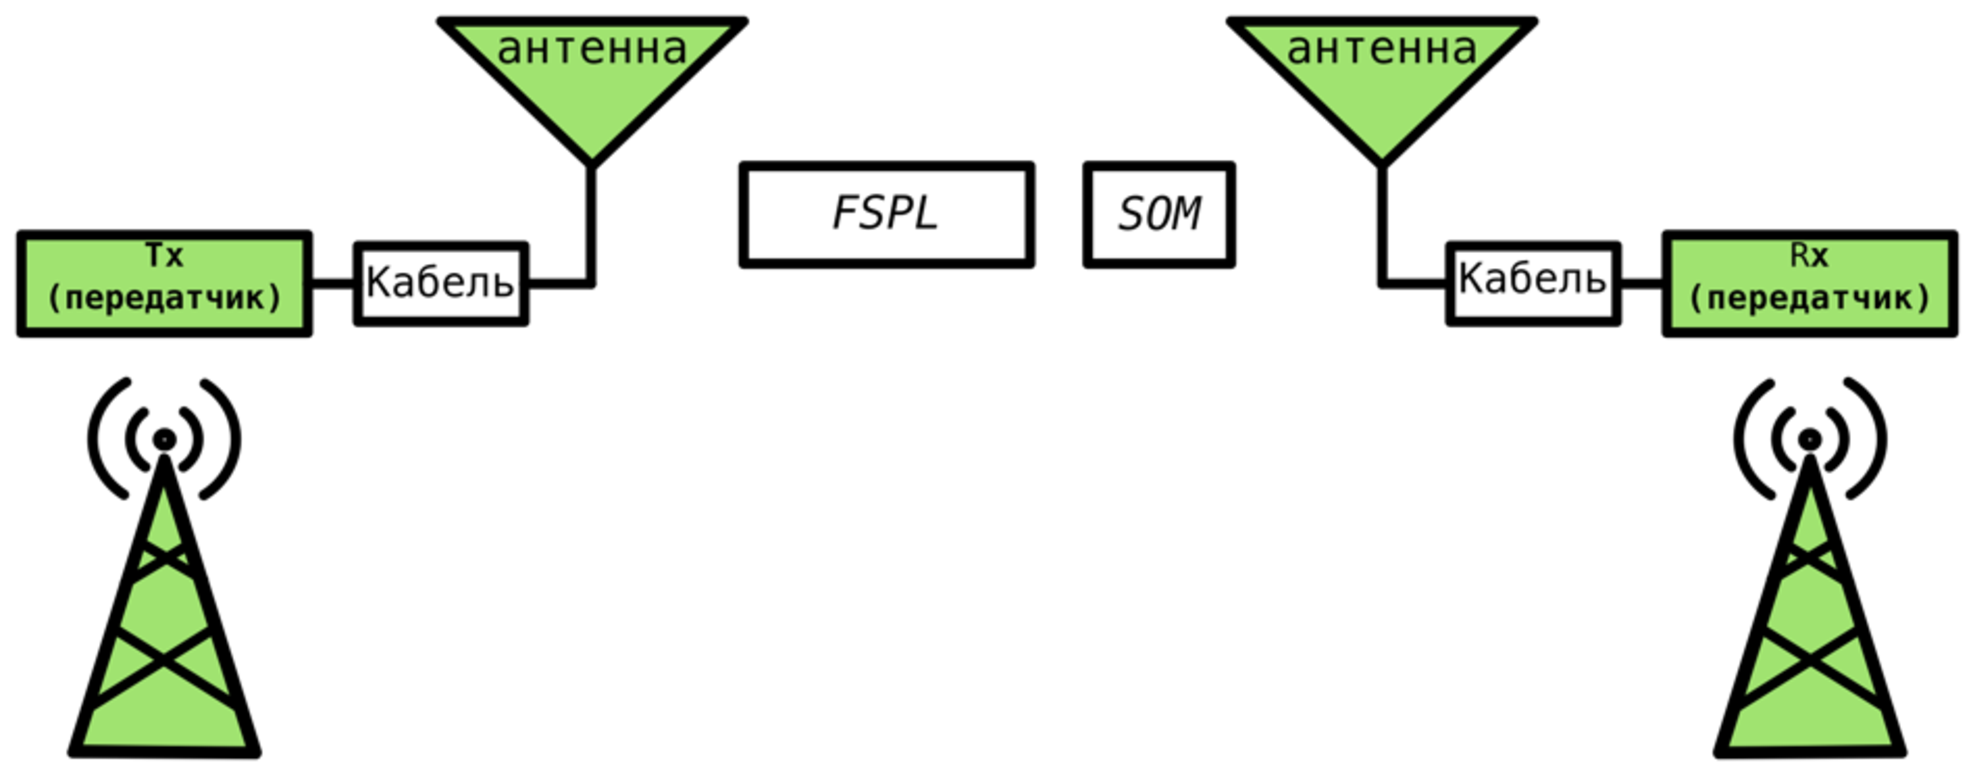
\includegraphics[width=0.8\textwidth]{link_distance.pdf}
% \caption{Соеденинение между станциями.}
% \label{fig:part3_link_distance}
% \end{figure}

% Для расчета дальности связи $R_{jq}$ (Рис. \cref{fig:part3_link_distance}), базовые станции $s_j$ и $s_q$ будут рассматриваться как станции \textit{передатчик} и \textit{приемник}, соответственно. Будем считать, что станции обрудованы направленными антеннами с усилениями $G_{tr}^{R}$ и $G_{recv}^{R}$.

% \begin{figure}[h!]
%   \centering
%    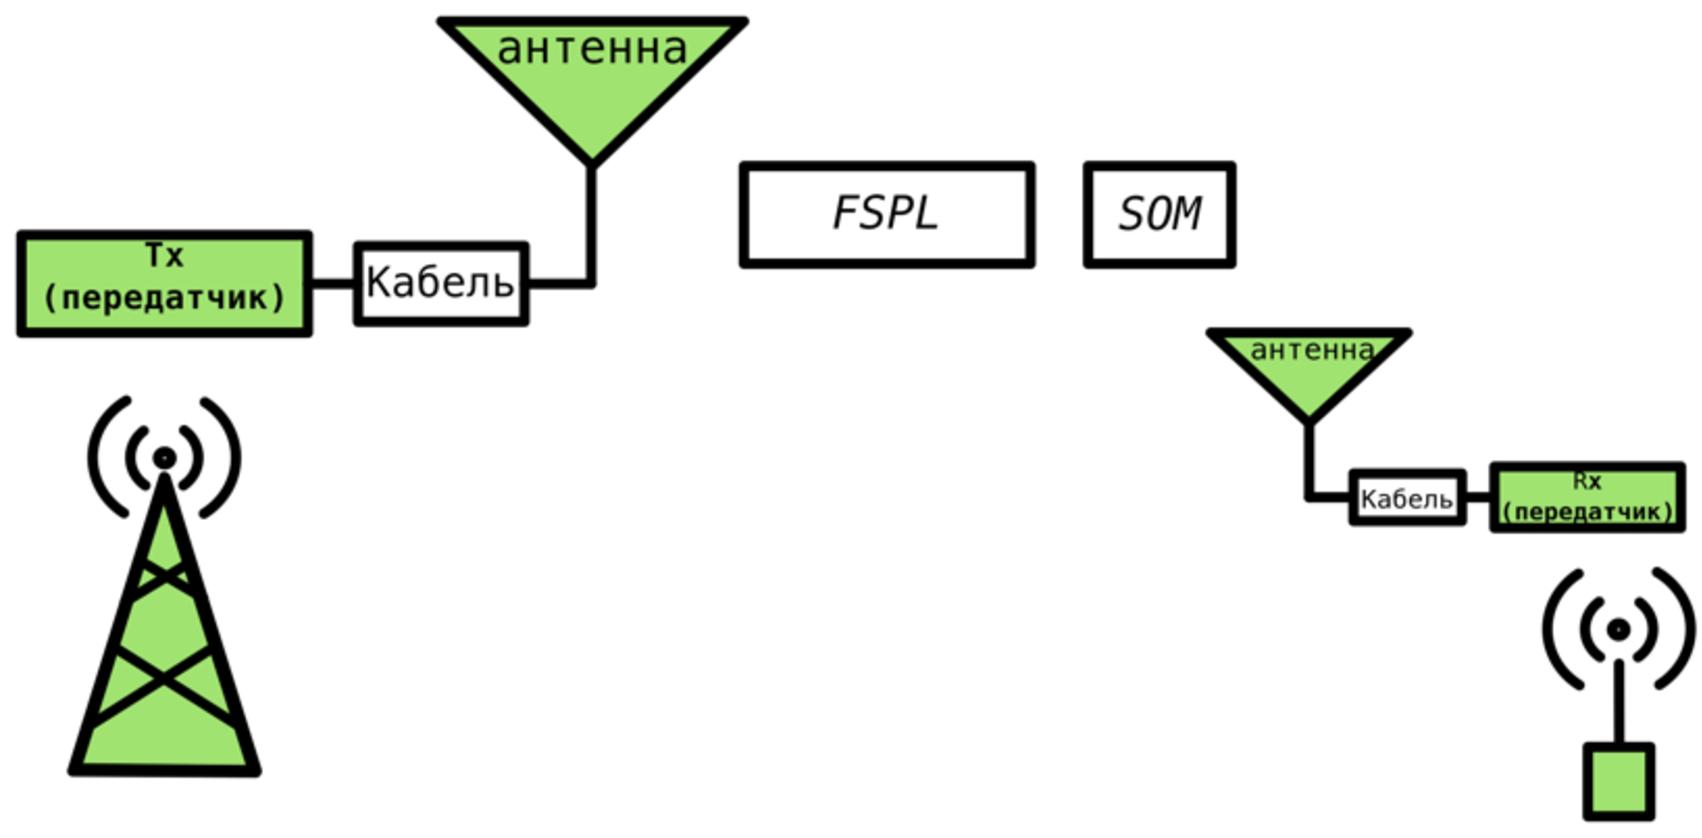
\includegraphics[width=0.8\textwidth]{coverage.pdf}
% \caption{Покрытие станции}
% \label{fig:part3_coverage}
% \end{figure}

% Каждая базовая станция оснащена всенаправленной антенной с заданным усилением антенны $G_ {tr}^{r}$. Данная антенн необходимо для покрытия заданной области.

% Each base station is equipped with an omnidirectional antenna with given gain antenna $G_{tr}^{r}$. A station uses this antenna to cover a given area.

% При вычислении радиуса покрытия $r_j$ (Рис.  \cref{fig:part3_coverage}) базовая станция будем считать \textit{передатчиком} а пользовательское устройство \textit{приемником}.

\section{Модель ЦЛП}

После оценки максимальных радиуса связи между станциями $R_{jq}$, максимального радиуса покрытия $r_j$, можно перейти, непосредственно, к задаче размещения станций в виде модели целочисленного линейного программирования.

Пусть $y_i^+$ и $y_i^-$ , $i= \overline{0,n+1}$ определяют охват покрытия (справа и слева, соответственно) станций, покрывающих точку $a_i$ (Рис. \cref{fig:part3_station_coverage}). Параметры $y_i^+$ и $y_i^-$ могут принимать только неотрицательные целые значения.

Величины  покрытия для шлюзов $y_0^+, y_0^-, y_{n+1}^+, y_{n+1}^-$ равны 0.

\begin{figure}[ht]
  \centerfloat{
      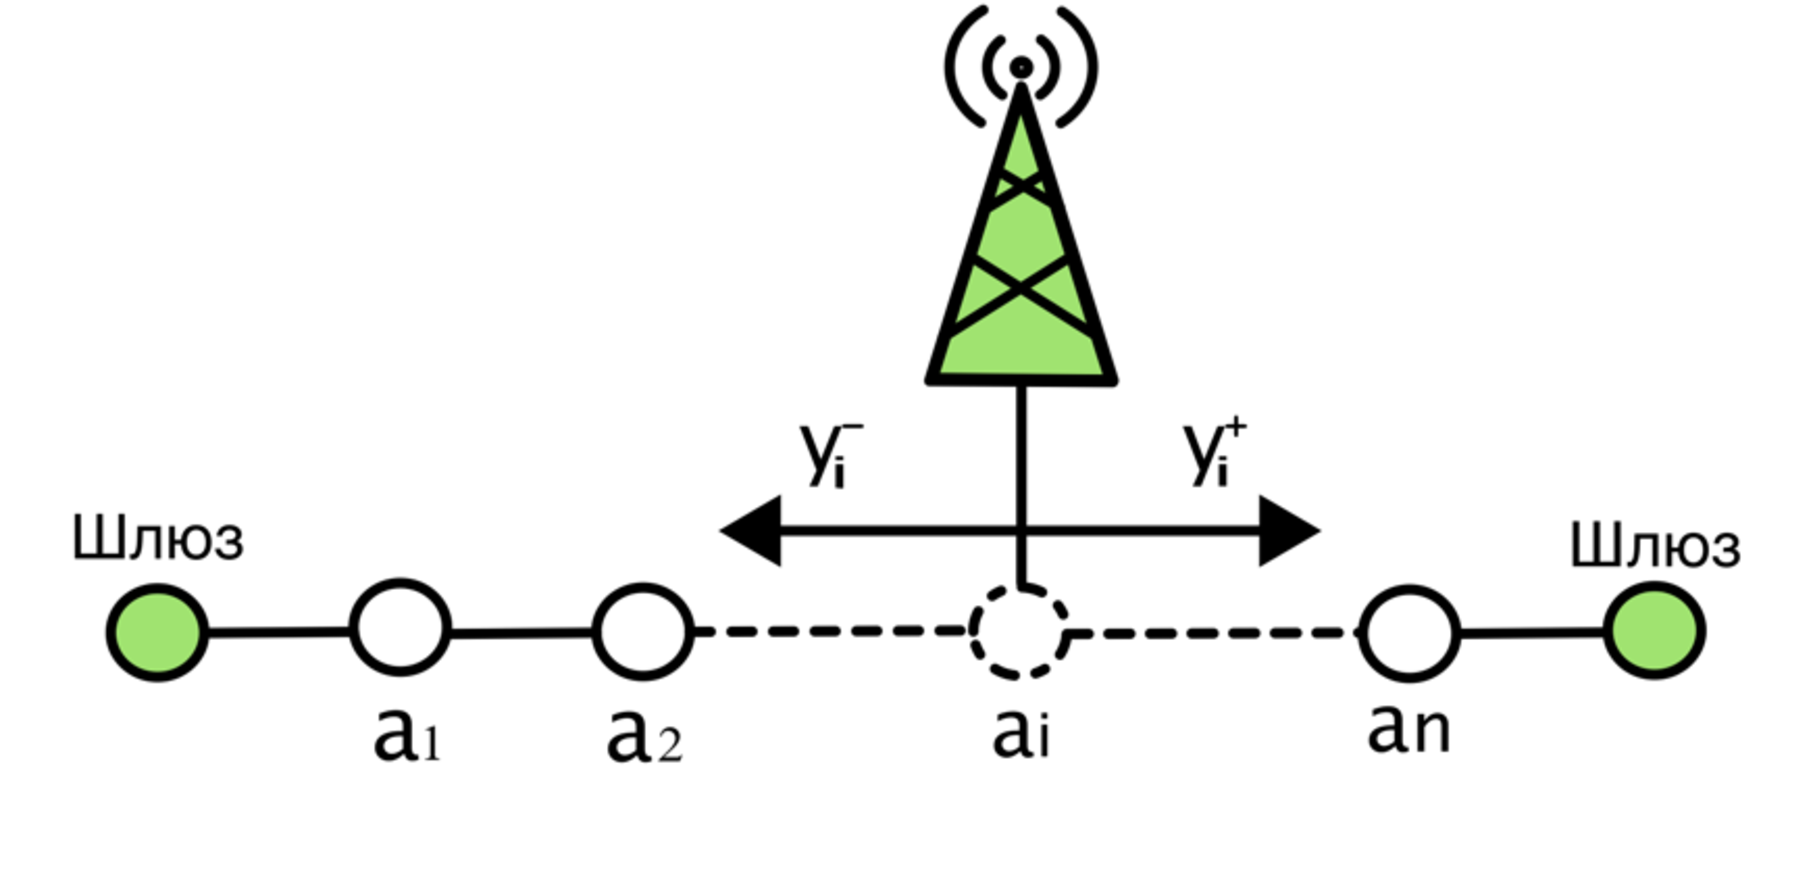
\includegraphics[scale=0.5]{station_coverage.pdf}
  }
  \caption{Охват покрытия станции]}\label{fig:part3_station_coverage}
\end{figure}

Целевая функция будет представлена как:
\begin{equation}
  \label{eq:part3_objective_function}
  f =  \sum\limits_{i=1}^n (y_i^- + y_i^+) \rightarrow max
\end{equation}

Также введем бинарные переменные $x_{ij}$. Тогда $x_{ij}=1$, если станция $s_j$, размещенная на точке $a_i$, и $x_{ij}=0$ в противном случае; $i= \overline{1, n}$; $j = \overline{1,m}$.

Введем двоичные переменные $ e_i $. Тогда $ e_i = 1 $, если какая-либо станция находится в точке $ a_i $, и $ e_i = 0$  в противном случае; $ i = \overline {1, n} $. Для точек размещения шлюзов $ a_0 $ и $a_{n + 1}$ переменные $ e_0 = 1 $ и $ e_{n + 1} =1 $, соответственно. 

% Let us introduce binary variables $e_i$. Then $e_i$  is equal to 1, if any station is placed at point $a_i$ and $e_i$ is equal to 0 otherwise; $i = \overline{1, n}$. For gateways placement points $e_0$  is equal to 1 and $e_{n+1}$  is equal to 1.

Сформулируем следующую систему ограничений задачи.

По определению \cref{eq:part3_ei}:

\begin{equation}
  \label{eq:part3_ei}
  e_i =  \sum\limits_{j=1}^m x_{ij}, \quad i = \overline{1,n}. 
\end{equation}

Каждая станция должна быть размещена только в одной точке. \cref{eq:part3_xij}:

\begin{equation}
  \label{eq:part3_xij}
  \sum\limits_{j=1}^n x_{ij} \leq 1, \quad j = \overline{1,m}. 
\end{equation}

Значения покрытий не превышают радиус покрытия станции, размещенной в точке $ a_i $, и равны 0, если в точке $a_i$  нет станции \cref{eq:part3_yi_1, eq:part3_yi_2}:


\begin{equation}
  \label{eq:part3_yi_1}
  y_i^+ \leq \sum\limits_{j=1}^m x_{ij} \cdot r_j, \quad i = \overline{1,n};
\end{equation}

\begin{equation}
  \label{eq:part3_yi_2}
  y_i^- \leq \sum\limits_{j=1}^m x_{ij} \cdot r_j, \quad i = \overline{1,n}. 
\end{equation}

Общая область покрытия между любыми двумя точками $ a_i $ и $ a_k $, где расположены станции, не может превышать расстояние между этими точками \cref{eq:part3_yi_3, eq:part3_yi_4}.

\begin{equation}
  \label{eq:part3_yi_3}
  y_i^+ + y_k^- \leq \frac{l_k - l_i}{2} \cdot (e_i + e_k ) + (2 - e_i - e_k ) \cdot L, \quad i = \overline{1,n},  \quad k = \overline{i+1,n+1};
\end{equation}

\begin{equation}
  \label{eq:part3_yi_4}
  y_i^- + y_k^+  \leq \frac{l_i-l_k}{2} \cdot (e_i + e_k) + (2 - e_i - e_k) \cdot L, \quad i = \overline{1,n}, \quad k = \overline{i-1,0},
\end{equation}
где $ l_k $ и $ l_i $ - координаты точек $ a_i $ и $ a_k $, соответственно. Это условие исключает влияние пересечений покрытий станций при вычислении общего значения покрытия между станциями (Рис. \cref{fig:part3_total_coverage_between_points}).

\begin{figure}[ht]
  \centerfloat{
      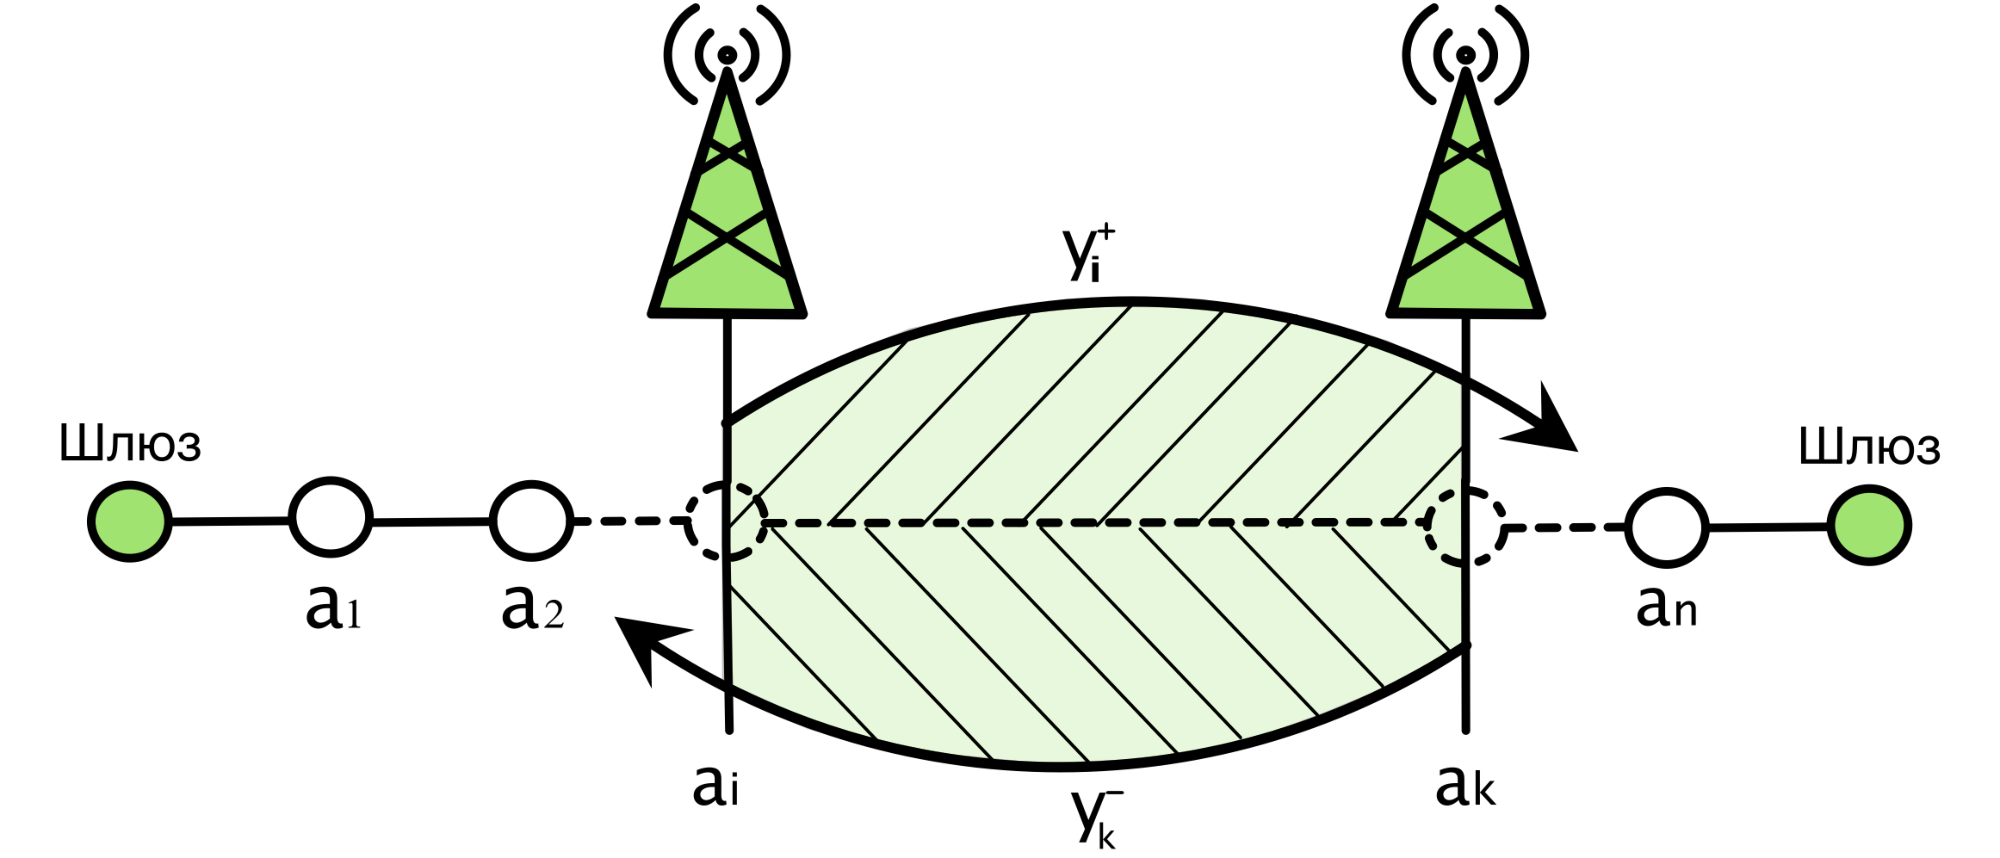
\includegraphics[scale=0.5]{total_coverage_between_points.pdf}
  }
  \caption{Область покрытия между любыми двумя точками}\label{fig:part3_total_coverage_between_points}
\end{figure}

Согласно условиям задачи, станция, расположенная в $ a_i $, должна быть связана хотя бы с одной станцией слева и одной станцией справа, включая станции на конечных точках $ a_0 $ и $a_{n + 1}$. 

Введем бинарные переменные $z_{ijkq}, i = \overline{1,n}; j= \overline{1,m}; k=\overline{1,n},  k \neq i; q= \overline{1,m}, q \neq j$.

Переменная $ z_ {ijkq} = 1$, если в точке $ a_i $ размещена станция $ s_j $ и данная станция связана со станцией $ s_q $, размещенная в точке $ a_k $; и $ z_ {ijkq} = 0 $ в противном случае.

Переменная $ z_{ij0(m + 1)} = 1$, если станция $ s_j $, размещенная в точке $ a_i $, связана со шлюзом $ s_{m + 1} $ в точке $ a_0 $; $ z_{ij0 (m + 1)} = 0 $ в противном случае.
 
Переменная $ z_{ij(n + 1)(m + 1)} = 1 $, если здесь находится станция $ s_j $ в точке $ a_i $ и она связана со шлюзом $ s_{m + 1} $ в точке $ a_{n + 1} $; $ z_{ij0(m + 1)} = 0 $  в противном случае.

Станции должны быть размещены в обеих точках $ a_i $ и $ a_k $, \cref{eq:part3_z_ijkq_1, eq:part3_z_ijkq_2}:

\begin{equation}
  \label{eq:part3_z_ijkq_1}
  z_{ijkq} \leq e_i , \quad i = \overline{1, n}; \quad j = \overline{1, m}; \quad k = \overline{1,n}, k \neq i; \quad q = \overline{1,m}, q \neq j;
\end{equation}


\begin{equation}
  \label{eq:part3_z_ijkq_2}
  z_{ijkq} \leq e_k , \quad k = \overline{1, n}; \quad j = \overline{1, m}; \quad i = \overline{1,n}, i \neq k; \quad q = \overline{1,m}, q \neq j.
\end{equation}


Необходимо, чтобы станция $ s_j $ в точке $ a_i $ была связана с  любой станцией, расположенной в точке $ a_k $, справа от $ a_i $ ($ k> i $) или с правым шлюзом $ s_{m + 1} $ \cref{eq:part3_z_ijkq_3_1, eq:part3_z_ijkq_3_2}. 

\begin{equation}
  \label{eq:part3_z_ijkq_3_1}
  \sum\limits_{k=i+1}^{n} \sum\limits_{\substack{q = 1\\ q \neq j}}^m z_{ijkq} + z_{ij(n+1)(m+1)} = x_{ij} ,  \quad i = \overline{1, n}, \quad j = \overline{1, m}.
\end{equation}


Станция $ s_j $, размещенная в $ a_{n} $, справа связана толко со шлюзом $ s_{m + 1} $ на месте $ a_ {n+1}$ \cref{eq:part3_z_ijkq_3_2}. 

\begin{equation}
  \label{eq:part3_z_ijkq_3_2}
  z_{nj(n+1)(m+1)} = x_{nj} \quad j = \overline{1, m}.
\end{equation}

Также станция должна быть связана с любой станцией, расположенной в точке $ a_k $ слева от точки $ a_i $ ($ k <i $) или с левым шлюзом $ s_{m + 1} $ \cref{eq:part3_z_ijkq_4_1, eq:part3_z_ijkq_4_2}.

\begin{equation}
  \label{eq:part3_z_ijkq_4_1}
  z_{1j0(m+1)}= x_{ij}, \quad j = \overline{1, m};
\end{equation}

Станция $s_j$, размещенная в точке $a_{1}$ слева может быть связана только со шлюзом $s_{m+1}$, расположенном в точке $a_0$ \cref{eq:part3_z_ijkq_4_1}.

\begin{equation}
  \label{eq:part3_z_ijkq_4_2}
  z_{ij0(m+1)} + \sum\limits_{k=1}^{i-1} \sum\limits_{\substack{q = 1\\ q \neq j}} z_{ijkq}= x_{ij}, \quad i = \overline{2, n}, \quad j = \overline{1, m}.
\end{equation}

Необходимо, чтобы станция $ s_q $ в точке $ a_k $ была связана с любой станцией справа, расположенной в точке $ a_i $ \cref{eq:part3_z_ijkq_5}.

\begin{equation}
  \label{eq:part3_z_ijkq_5}
  \sum\limits_{i=k+1}^{n} \sum\limits_{\substack{j=1 \\ j \neq q}}^m z_{ijkq} = x_{kq} , \quad k = \overline{1, n-1}, \quad q = \overline{1, m};
\end{equation}

Кроме того, станция $ s_q $ в точке $ a_k $ подключена к любой станции слева, расположенной в точке $ a_i $ \cref {eq:part3_z_ijkq_6}. 

\begin{equation}
  \label{eq:part3_z_ijkq_6}
  \sum\limits_{i=1}^{k} \sum\limits_{\substack{j=1 \\ j \neq q}}^m z_{ijkq} = x_{kq} , \quad k = \overline{2, n}, \quad q = \overline{1, m};
\end{equation}

Неравенства \cref{eq:part3_z_ijkq_1, eq:part3_z_ijkq_2} и равенства \cref{eq:part3_z_ijkq_3_1, eq:part3_z_ijkq_3_2, eq:part3_z_ijkq_4_1, eq:part3_z_ijkq_4_2, eq:part3_z_ijkq_5, eq:part3_z_ijkq_6} обеспечивают условие симметрии связи между базовыми станциями, расположенными в точках $ a_i $ и $ a_k $, $\forall i, k $ (Рис.\cref{fig:part3_station_link}).

\begin{figure}[ht]
  \centerfloat{
      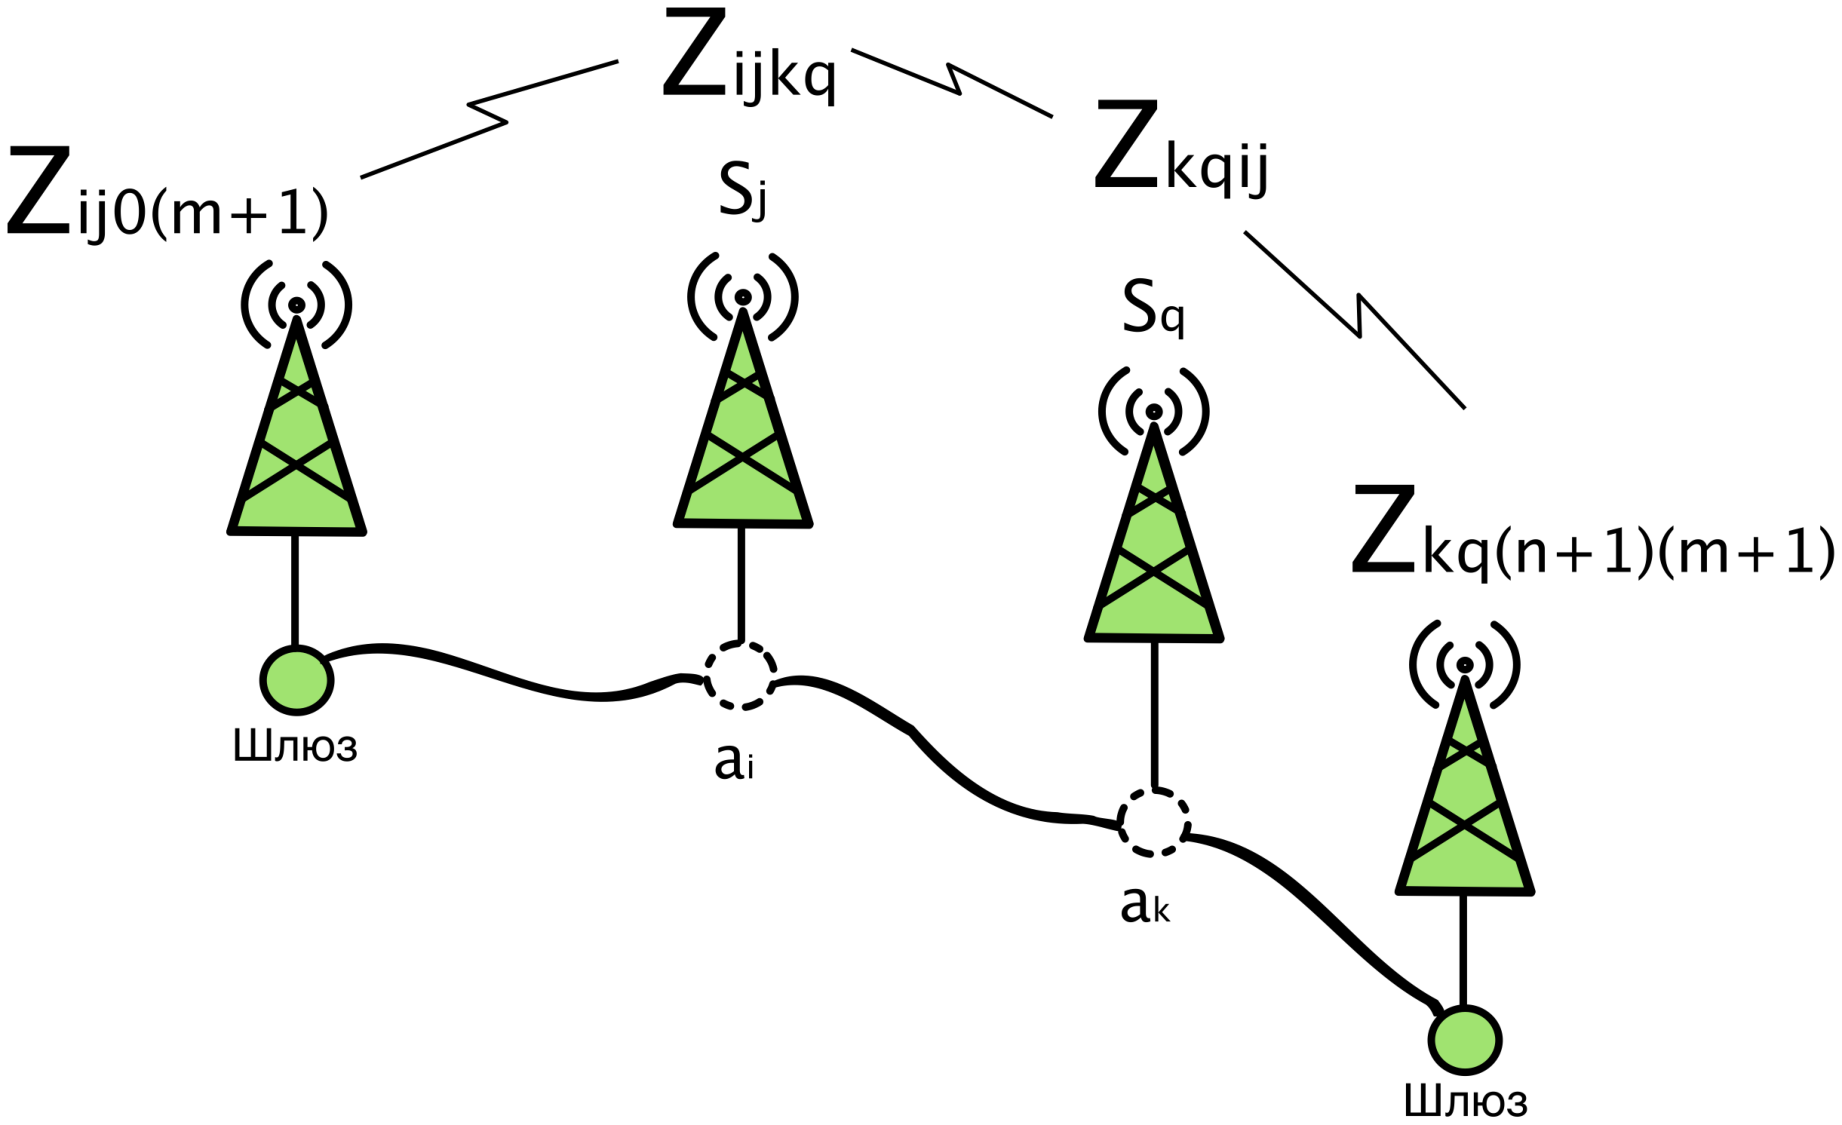
\includegraphics[scale=0.5]{station_link.pdf}
  }
  \caption{Связь между базовыми станциями}\label{fig:part3_station_link}
\end{figure}

Если станции $ s_j $ и $ s_q $ связаны, то максимальноый радиус связи размещенных станций должен быть не меньше расстояния между точками $ a_i $ и $ a_k $, где расположены станции $ s_i $ и $ s_q $ (Рис. \cref{fig:part3_station_link_between_points}). Формально это можно записать как \cref{eq:part3_z_ijkq_7, eq:part3_z_ijkq_8}.

 $\forall i= \overline{1,n}$:
\begin{equation}
  \label{eq:part3_z_ijkq_7}
  z_{ijkq}(R_{jq}-(a_i-a_k ))\geq 0, \quad k=\overline{0,i-1}; \quad j=\overline{1,m}; \quad q= \overline{1,m}, q \neq j; 
\end{equation}

\begin{equation}
  \label{eq:part3_z_ijkq_8}
  z_{ijkq} (R_{jq}-(a_k-a_i )) \geq 0, \quad k=\overline{i+1,n+1}; \quad j=\overline{1,m}; \quad q= \overline{1,m}, q \neq j.
\end{equation}

\begin{figure}[ht]
  \centerfloat{
      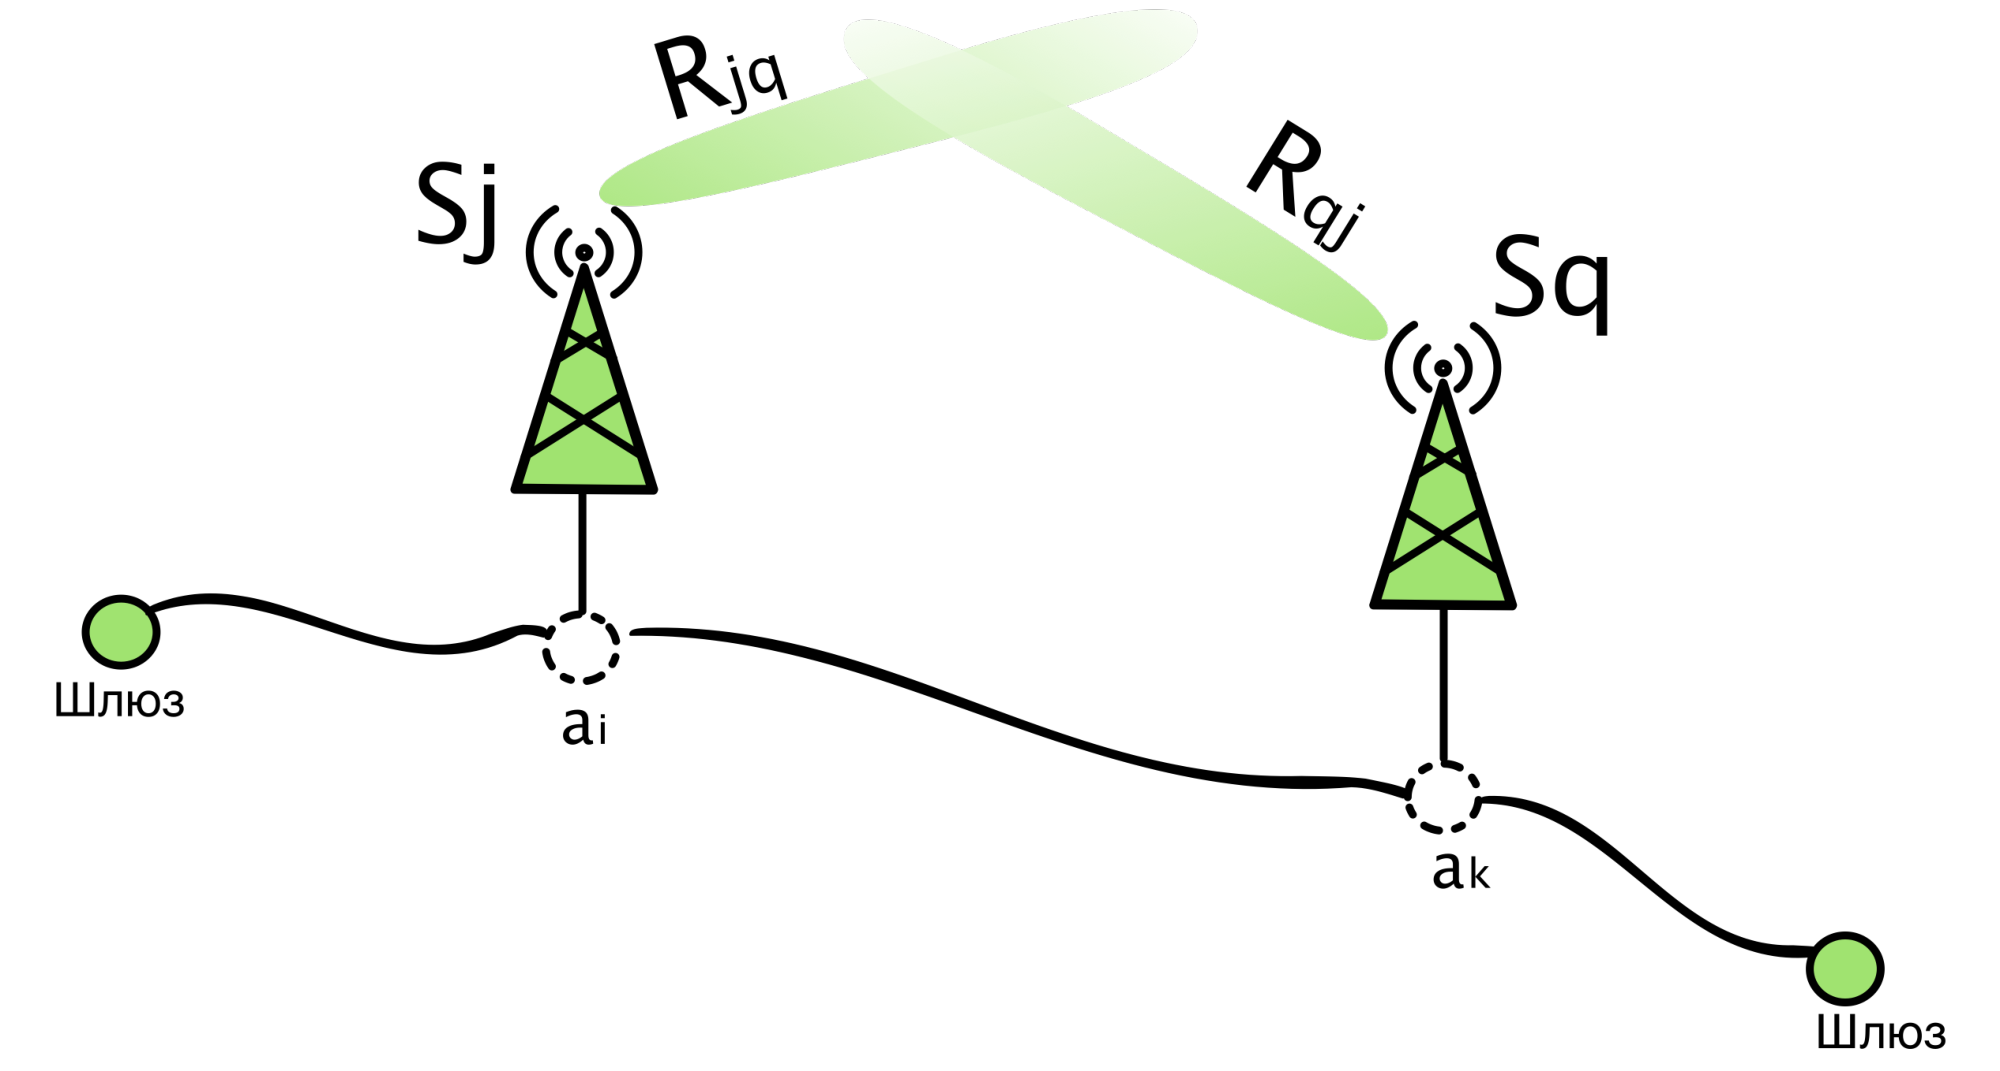
\includegraphics[scale=0.5]{station_link_between_points.pdf}
  }
  \caption{Обеспечение связи с соседней станцией}\label{fig:part3_station_link_between_points}
\end{figure}

И для бюджетного ограничения стоимости $C$:

\begin{equation}
  \label{eq:part3_cost}
  \sum\limits_{i=1}^n \sum\limits_{j=1}^m x_{ij} \cdot c_j \leq C.
\end{equation}


\section{Численный пример}
В этой секции представлен численный пример решения данной задачи.
% This section shows one simple case of the problem.

Задан линейный участок $L$ с длиной 300 с количеством $n=7$ точек размещения. Координаты точек размещения представлены в таблице \cref{tab:part3_placed_point}.  Задан бюджет размещения $C=130$. Центарльная частота $f = 2437$ МГц. 

\begin{table}[h!]\centering
  \begin{tabular}{|c||c|c|c|c|c|c|c|}\hline
    $a_i$ & $a_1$ &  $a_2$ & $a_3$ & $a_4$ & $a_5$ & $a_6$ & $a_7$ \\ \hline \hline
    Координата & 29 & 40 & 95 & 139 & 181 & 230 & 273 \\ \hline
\end{tabular}\caption{Точки размещения участка с длиной $L = 300$.}\label{tab:part3_placed_point}
\end{table}

Задано множества базовых станций $m = 8$ с параметрами представленными в таблице \cref{tab:part3_BS}. Также в таблице представлены параметры шлюзов и контролируемых объектов. Параметры объектов необходимы для расчета радиусов покрытия станций.

\begin{table}[b]\centering
  \begin{tabular}{|c||c|c|c|c|c|c|c|}\hline
    BS & $P_{tr}^R$ &  $G_{tr}^R$ & $P_{recv}^R$ & $P_{recv}^r$ & $G_{recv}^r$ & $c$ \\ \cline{2-1} \cline{3-1} \cline{4-1} \cline{5-1}  \cline{6-1} \cline{7-1}
     & дБм & дБ & Дбм & дБм & дБ & у.е.  \\ \hline
    1 & 20 & 5 & -69 & -67 & 5 & 40 \\ 

    2 & 19 & 5 & -67 & -67 & 5 & 28 \\ 

    3 & 18 & 5 & -69 & -67 & 5 & 45 \\ 

    4 & 19 & 5 & -69 & -67 & 6 & 22 \\ 

    5 & 19 & 5 & -67 & -67 & 5 & 21 \\ 

    6 & 20 & 5 & -69 & -67 & 5 & 40 \\ 

    7 & 19 & 5 & -67 & -67 & 5 & 28 \\

    8 & 18 & 5 & -69 & -67 & 5 & 45 \\ \hline \hline  

    &  $G_{recv}^R$ & $P_{recv}^R$ &  & & $P_{tr}^r$ & $G_{tr}^r$ \\  \cline{2-1} \cline{3-1} \cline{6-1} \cline{7-1} 

    Шлюз& дБ & дБм & & Объект & дБм & дБ  \\  \cline{2-1} \cline{3-1}  \cline{6-1} \cline{7-1}

    &  5 & -69 & &  & 15 & 2  \\ \hline

  \end{tabular}\caption{Параметры базовых станций, шлюзов и объектов.}\label{tab:part3_BS} 
\end{table}

\subsection{Расчет радиса связи между станциями}
Базовые станции оснащены направленной антенной с высоким коэффициентом усиления для связи с соседними станциями.
Для расчета потерь между станциями $j$ и $q$ воспользуемся формулой (\ref{eq:part3_L_fs_from_link_budget}):

\begin{displaymath}
  L_{fs}^{jq} = P_{tr}^R(j) - L_{tr} + G_{tr}^R(j) + G_{tr}^R(q) - L_{recv} - SOM - P_{recv}^R(q).
\end{displaymath}


Потери на кабелях приемникп $ L_{recv} $ и передатчике $ L_{tr} $ примем равным 1 дБ и запас на замирания сигнала $ SOM = 10 $ дБ.

Let us carry out an example of the calculation communication link between stations $ s_1 $ and $ s_2 $:
Для примера расчетаем радиус связи между станциями $ s_1 $ и $ s_2 $:

\begin{align}
  \begin{aligned}
  L_{fs}^{12} = P_{tr}^R(1) - L_{tr} + G_{tr}^R(1) + G_{tr}^R(2) - L_{recv} - SOM - P_{recv}^R(2)= \\
  = 20 - 1 + 5 + 5 - 1 - 10 - (-69) = 87 (dB).
  \end{aligned}
\end{align}

Для расчета канала связи необходимо использовать формулу \cref{eq:part3_D}. Несущая частота $ f = 2437 $ МГц и коэффициент для расчета потерь $ K = -27,55 $:

\begin{align}
  \begin{aligned}
  R_{jq} = 10^{\left(\frac{L_{fs}^{jq} - 20\lg{F} - K}{20}\right)}
  = 10^{\left(\frac{87 - 20\lg{2437} - (-27.55)}{20}\right)} = 174 (m).
  \end{aligned}
\end{align}

В таблице \cref{tab:part3_Rjq} приведены расчеты максимальных радиусов связи между всеми станциями $ s_j $, $ j = 1, ..., m $ и шлюзом $ s_ {m + 1} $.

\begin{table}[h!]\centering
  \begin{tabular}{|c||c|c|c|c|c|c|c|c|c|}\hline
      $R_{jq}, (m)$ & $s_1$ & $s_2$ & $s_3$ & $s_4$ & $s_5$ & $s_6$ & $s_7$ & $s_8$ & $s_{m+1}$ \\ \hline \hline

      $s_1$ &--& 174& 219& 219& 174& 219& 174& 219& 219\\ 
      $s_2$ &195& --& 195& 195& 155& 195& 155& 195& 195\\ 
      $s_3$ &174& 138& --& 174& 138& 174& 138& 174& 174\\ 
      $s_4$ &195& 155& 195& --& 155& 195& 155& 195& 195\\ 
      $s_5$ &195& 155& 195& 195& --& 195& 155& 195& 195\\ 
      $s_6$ &219& 174& 219& 219& 174& --& 174& 219& 219\\
      $s_7$ &195& 155& 195& 195& 155& 195& --& 195& 195\\ 
      $s_8$ &174& 138& 174& 174& 138& 174& 138& --& 174\\ 
      \hline

\end{tabular}\caption{Рассчитанные радиусы связи между станциями}\label{tab:part3_Rjq}
\end{table}

\subsection{Расчет радиуса покрытия}

% Для покрытия заданного участка базовая станция оснащена всенаправленной антенной с выходной мощностью $ P_{tr}^r $ и усилением $ G_{tr}^r$. Потери в кабеле $ L_ {tr} $ равно 1.

% To cover a given section, the base station is equipped with an isotropic antenna with output power $ P_ {tr} ^ r $ and gain $ G_ {tr} ^ r $ is equal to 0. The cable loss $ L_ {tr} $ is equal to 1.

% A coverage area depends on a base station, as well as user device characteristics. Let us consider a user device with an antenna sensitivity $P_{RX} = -67$ dBm and gain $G_{RX} = 0$. Loss $L_{RX}$ is equal to 0.
Расчет проводится аналогично расчета радиусу связи между станциями. 
Потери в свободном простанстве для канала между $j$-ой станции и контролируемым объектом

\begin{displaymath}
  L_{fs}^{j} = P_{tr}^r(j) - L_{tr}  - SOM - P_{RX}. 
\end{displaymath}


Пример расчечта радиуса покрытия для  $1$-ой станции:

\begin{displaymath}
  L_{fs}^{1} = P_{tr}^r + G_{tr}^r + G_{recv}^r(1) - L_{recv}(1)  - SOM - P_{recv}^r(1) = 15+2+5-1-(-67)-10 = 78 \text{ (дБ)}.
\end{displaymath}

\begin{displaymath}
  r_{1} = 10^{\left(\frac{78 - 20\lg{2437} - (-27.55)}{20}\right)} = 77 \text{ (м)}.
\end{displaymath}

Рассчитанные радиусы покрытия для всех станций $ s_j $, $ j = \overline{1, m} $ представлены в таблице \cref{tab:part3_rj}).

\begin{table}[h!]\begin{center}
  \begin{tabular}{|c||c|c|c|c|c|c|c|c|}\hline
      STA & $s_1$ & $s_2$ & $s_3$ & $s_4$ & $s_5$ & $s_6$ & $s_7$ & $s_8$\\ \hline \hline

      $r_{j}$ & 77 & 77 & 77 & 87 & 77 & 77 & 77 & 77\\ \hline

\end{tabular}\caption{Рассчитанные радиусы покрытия станций}\label{tab:part3_rj}
\end{center}\end{table}

Задача ЦЛП решена с помощью Optimization Toolbox MatLab. Таблица \cref{tab:part3_ilp_solution} содержит все возможные целочисленные решения.

\begin{table}[h!]\centering
  \begin{tabular}{|c||c|c|c|c|c|c|c||c|c|}\hline
    $a_i$ & $a_1$ &  $a_2$ & $a_3$ & $a_4$ & $a_5$ & $a_6$ & $a_7$  & Покрытие & Цена \\ \hline 
    Координаты & 29 & 40 & 95 & 139 & 181 & 230 & 273 & м & у.е.\\ \hline \hline
    Целлочисленное решение 1 & $s_1$ & $s_2$ & $s_6$ & -- & -- & -- & $s_4$ & 286 & 130\\ 
    Целлочисленное решение 2 & $s_4$ & -- & $s_5$ & $s_7$ & -- & -- & $s_2$ & 289 & 99\\
    Оптимальное решение & $s_4$ & $s_2$ & -- & -- & $s_1$ & -- & $s_5$ & 300 & 111 \\ \hline
\end{tabular}\caption{Решение задачи ЦЛП.}\label{tab:part3_ilp_solution}
\end{table}

\section{Выводы по Главе \cref{chapter_ilp_model}}
Представлена математическая модель задачи размещения базовых станций беспроводной сети связи вдоль линейного участка в виде задачи ЦЛП. В качестве примера представлен численный пример решения задачи.

% \section{Example}

% Let's look at one simple case of base stations placement problem.

% Consider the section of length $L = 400$ with $n = 10$ placement points is given in table \ref{tab:placed_point}:

% \begin{table}[h!]\begin{center}
%   \begin{tabular}{|c||c|c|c|c|c|c|c|c|c|c|}\hline
%     $a_i$ & $a_1$ &  $a_2$ & $a_3$ & $a_4$ & $a_5$ & $a_6$ & $a_7$ & $a_8$ & $a_9$ & $a_{10}$ \\ \hline \hline
%     coordination & 32 & 65 & 101 & 142 & 181 & 241 & 270 & 301 & 325 & 380 \\ \hline
% \end{tabular}\caption{Placement points at the section of length $L = 400$.}\label{tab:placed_point}
% \end{center}\end{table}

% There are $m = 7$ base stations with parameters given in table \ref{tab:BS}:

% \begin{itemize}
%   \item $P_{tr}^R$ is a transmit power for communication with base stations;
%   \item $G_{tr}^R$ is an antenna gain for communication with base stations;
%   \item $P_{recv}^R$ is a sensitivity for communication with base stations;
%   \item $P_{tr}^r$ is a transmit power for the coverage of section;
%   \item $G_{tr}^r$ is an antenna gain for the coverage of section;
%   \item $p$ is a throughput;
%   \item $c$ is a base station cost.
% \end{itemize}

% \begin{table}[h!]\begin{center}
%   \begin{tabular}{|c||c|c|c|c|c|c|c|}\hline
%     BS & $P_{tr}^R$ &  $G_{tr}^R$ & $P_{recv}^R$ & $P_{tr}^r$ & $G_{tr}^r$ & $p$ & $c$ \\ \hline 
%     No & [dBm] & [dBi] & [dBm] & [dBm] & [dBi] & Mbit/s & c.u.  \\ \hline
%     1 & 19 & 5 & -69 & 20 & 2 & 54 & 2300 \\ 

%     2 & 19 & 4 & -80 & 19 & 3 & 54 & 1200 \\ 

%     3 & 19 & 6 & -69 & 18 & 2 & 54 & 4500 \\ 

%     4 & 19 & 5 & -83 & 18 & 3 & 54 & 6000 \\ 

%     5 & 20 & 5 & -85 & 20 & 2 & 54 & 3500 \\ 

%     6 & 22 & 5 & -69 & 18 & 2 & 54 & 4200 \\ 

%     7 & 19 & 5 & -69 & 18 & 2 & 54 & 4200 \\ \hline

% \end{tabular}\caption{Base station parameters.}\label{tab:BS}
% \end{center}\end{table}

% Finally, gateway stations of special type $s_{m + 1}$ placed on the ends of the segment are specified. Gateway parameters is given in table \ref{tab:Gateway}:

% \begin{table}[h!]\begin{center}
%   \begin{tabular}{|c||c|c|}\hline
%     Gateway & $G_{tr}^R$ & $P_{recv}^R$  \\ \hline 
%      No & [dBi] & [dBm]  \\ \hline
%     $s_{m+1}$ & 3 & -69 \\ \hline

% \end{tabular}\caption{Gateway parameters.}
% \label{tab:Gateway}
% \end{center}\end{table}

% \subsection{Computation of the communication link distance between base stations}

% Base station is equipped with a directional antenna with a high gain to communicate with neighbouring stations.
% To calculate the losses between stations $j$ and $q$, we use the formula (\ref{eq:L_fs_from_link_budget}):

% \begin{displaymath}
%   L_{fs}^{jq} = P_{tr}^R(j) - L_{tr} + G_{tr}^R(j) + G_{tr}^R(q) - L_{recv} - SOM - P_{recv}^R(q).
% \end{displaymath}

% The cable losses at the receiver $L_{recv}$ and transmitter $L_{tr}$ are equal to 1 dB. We will also provide system operating margin $ SOM = 10 $ dB.

% Let us carry out an example of the calculation communication link between stations $ s_1 $ and $ s_2 $:

% \begin{align}
%   \begin{aligned}
%   L_{fs}^{12} = P_{tr}^R(1) - L_{tr} + G_{tr}^R(1) + G_{tr}^R(2) - L_{recv} - SOM - P_{recv}^R(2)= \\
%   = 19 - 1 + 5 + 4 - 1 - 10 - (-80) = 96 (dB).
%   \end{aligned}
% \end{align}

% To calculate the communication link, formula ( \ref{eq:D} ) must be used. The stations operate on 6th channel, carrier frequency $f = 2437$ MHz and coefficient $K = -27.55$:

% \begin{align}
%   \begin{aligned}
%   R_{jq} = 10^{\left(\frac{L_{fs}^{jq} - 20\lg{F} - K}{20}\right)}
%   = 10^{\left(\frac{96 - 20\lg{2437} - (-27.55)}{20}\right)} = 617 (m).
%   \end{aligned}
% \end{align}

% Table \ref{tab:Rjq} summarizes the maximal communication link distances calculations between all stations $ s_j $, $ j = 1, ..., m $, and the gateway $ s_ {m + 1} $.

% \begin{table}[h!]\begin{center}
%   \begin{tabular}{|c||c|c|c|c|c|c|c|c|}\hline
%       $R_{jq}, (m)$ & $s_1$ & $s_2$ & $s_3$ & $s_4$ & $s_5$ & $s_6$ & $s_7$ & $s_{m+1}$ \\ \hline \hline

%       $s_1$ & -- & 617 & 219 & 978 & 1 232 & 195 & 195 & 123 \\ 

%       $s_2$ & 174 & -- & 195 & 872 & 1 098 & 174 & 174 & 109 \\

%       $s_3$ & 219 & 692 & -- & 1098 & 1 382 & 219 & 219 & 138 \\

%       $s_4$ & 195 & 617 & 219 & -- & 1 232 & 195 & 195 & 123 \\

%       $s_5$ & 219 & 692 & 245 & 1 098  &  -- & 219 & 219 & 138 \\

%       $s_6$ & 275 & 872 & 309 & 1 382 &  1 740 & -- & 275 & 174 \\

%       $s_7$ & 195 & 617 & 219 & 978 & 1 232 & 195 & -- & 123 \\ \hline

% \end{tabular}\caption{The calculation of communication link distance between stations.}\label{tab:Rjq}
% \end{center}\end{table}


% \subsection{Computation of the coverage radius}

% To cover a given section, the base station is equipped with an isotropic antenna with output power $ P_ {tr} ^ r $ and gain $ G_ {tr} ^ r $ is equal to 0. The cable loss $ L_ {tr} $ is equal to 1.

% A coverage area depends on a base station, as well as user device characteristics. Let us consider a user device with an antenna sensitivity $P_{RX} = -67$ dBm and gain $G_{RX} = 0$. Loss $L_{RX}$ is equal to 0.

% Free space path loss between the $j$-th station and the user device

% \begin{displaymath}
%   L_{fs}^{j} = P_{tr}^r(j) - L_{tr}  - SOM - P_{RX}. 
% \end{displaymath}

% To calculate the coverage radius, must be used the formula (\ref{eq:D}). The stations operate on 6th channel, carrier frequency $f = 2437$ MHz. and coefficient $K = -27.55$

% \begin{displaymath}
%   r_{j} = 10^{\left(\frac{L_{fs}^{j} - 20\lg{F} - K}{20}\right)}.
% \end{displaymath}

% An example of calculating the coverage radius for the $1$-st station:

% \begin{displaymath}
%   r_{1} = 10^{\left(\frac{20 - 1 + 2 - 10 -(-67) - 20\lg{2437} - (-27.55)}{20}\right)} = 77 (m)
% \end{displaymath}

% Let's calculate the coverage radius for all stations $s_j $, $ j = 1, ..., m$ (table \ref{tab:rj}).

% \begin{table}[h!]\begin{center}
%   \begin{tabular}{|c||c|c|c|c|c|c|c|}\hline
%       STA & $s_1$ & $s_2$ & $s_3$ & $s_4$ & $s_5$ & $s_6$ & $s_7$ \\ \hline \hline

%       $r_{j}$ & 77 & 77 & 61 & 69 & 77 & 61 & 61 \\ \hline

% \end{tabular}\caption{Calculation of the coverage radius of stations.}\label{tab:rj}
% \end{center}\end{table}

% \subsection{Time delay calculation}

% Let's calculate the delay for station $s_1$. The specified throughput is $p_1 = 54$ Mbit/s. Let's assume that the average package size is $w = 2700$ KByte (21.6 MBit). The arrival package rate is $\lambda = 0.5(s^{- 1})$. Then the service rate according to the formula (\ref{eq:service_time}) will be

% \begin{displaymath}
%   \label{eq:service_time_evaluation}
%   \mu_1 = \frac{54}{21.6} = 2.5 (s^{-1}).
% \end{displaymath}

% The utilization is equal to

% \begin{displaymath}
%   \label{eq:rho_evaluation}
%   \rho_1 = \frac{0.5}{2.5} = 0.2.
% \end{displaymath}

% The average package size is

% \begin{displaymath}
%   \label{eq:N_evaluation}
%   \overline N_1 = \frac{0.2}{1 - 0.2} = 0.25.
% \end{displaymath}

% The average delay is

% \begin{displaymath}
%   \label{eq:node_delay_evaluation}
%   \overline {T_1} = \frac{0.25}{0.5} = 0.5 (s).
% \end{displaymath}

% Communication links between stations $R_{jq}$, the coverage radius of the station is $r_j$, the delays $\overline{T_j}$ are calculated, it is possible to search the optimal placement.

% The problem formulated on the basis of (\ref{eq:objective_function}) - (\ref{ineq:cost}) and given constraints on the cost $C = 18000$ and end-to-end delay $T = 3$ was solved by MATLAB Optimization Toolbox.

% The optimal placement is presented in the table \ref{tab:solution}.

% \begin{table}[h!]\begin{center}
%   \begin{tabular}{|c||c|c|c|c|c|c|c|c|c|c|} \hline
      
%       Placed station & $s_6$ & $s_7$ & -- & -- & $s_2$ & -- &  $s_5$ & -- & $s_1$ & -- \\ \hline

%       Placement coordination & $a_1$ &  $a_2$ & $a_3$ & $a_4$ & $a_5$ & $a_6$ & $a_7$ & $a_8$ & $a_9$ & $a_{10}$ \\  \hline

% \end{tabular}\caption{Solution result.}\label{tab:solution}
% \end{center}\end{table}
% Obtained total coverage $f$ is equal to 400 (m) with total cost $c$ is equal to $15400$ (c.u.), and end-to-end delay $T$ is equal to $ 2.5$ (s).

% \section{Conclusion}
% The paper considers the problem of finding an optimal placement of the given redundant set of base stations of wireless broadband communication network on a set of possible placement points to maximize the coverage area while respecting technological conditions and budget constraints.

% To calculate a limit on the network delay time a network is considered as a tandem queue model with $M/M/1$  nodes.

% The problem is formulated in the form of the integer linear programming model. Numerical example solution was presented.

% It is planned to use the obtained model in practice in future work.




% \bibliographystyle{splncs04}
% \bibliography{mukhtarov}

% \end{document}


% \section{Таблица обыкновенная}\label{sec:ch3/sect1}

% Так размещается таблица:

% \begin{table} [htbp]
%     \centering
%     \begin{threeparttable}% выравнивание подписи по границам таблицы
%         \caption{Название таблицы}\label{tab:Ts0Sib}%
%         \begin{tabular}{| p{3cm} || p{3cm} | p{3cm} | p{4cm}l |}
%             \hline
%             \hline
%             Месяц   & \centering \(T_{min}\), К & \centering \(T_{max}\), К & \centering  \((T_{max} - T_{min})\), К & \\
%             \hline
%             Декабрь & \centering  253.575       & \centering  257.778       & \centering      4.203                  & \\
%             Январь  & \centering  262.431       & \centering  263.214       & \centering      0.783                  & \\
%             Февраль & \centering  261.184       & \centering  260.381       & \centering     \(-\)0.803              & \\
%             \hline
%             \hline
%         \end{tabular}
%     \end{threeparttable}
% \end{table}

% \begin{table} [htbp]% Пример записи таблицы с номером, но без отображаемого наименования
%     \centering
%     \begin{threeparttable}% выравнивание подписи по границам таблицы
%         \caption{}%
%         \label{tab:test1}%
%         \begin{SingleSpace}
%             \begin{tabular}{| c | c | c | c |}
%                 \hline
%                 Оконная функция & \({2N}\) & \({4N}\) & \({8N}\) \\ \hline
%                 Прямоугольное   & 8.72     & 8.77     & 8.77     \\ \hline
%                 Ханна           & 7.96     & 7.93     & 7.93     \\ \hline
%                 Хэмминга        & 8.72     & 8.77     & 8.77     \\ \hline
%                 Блэкмана        & 8.72     & 8.77     & 8.77     \\ \hline
%             \end{tabular}%
%         \end{SingleSpace}
%     \end{threeparttable}
% \end{table}

% Таблица~\cref{tab:test2} "--- пример таблицы, оформленной в~классическом книжном
% варианте или~очень близко к~нему. \mbox{ГОСТу} по~сути не~противоречит. Можно
% ещё~улучшить представление, с~помощью пакета \verb|siunitx| или~подобного.

% \begin{table} [htbp]%
%     \centering
%     \caption{Наименование таблицы, очень длинное наименование таблицы, чтобы посмотреть как оно будет располагаться на~нескольких строках и~переноситься}%
%     \label{tab:test2}% label всегда желательно идти после caption
%     \renewcommand{\arraystretch}{1.5}%% Увеличение расстояния между рядами, для улучшения восприятия.
%     \begin{SingleSpace}
%         \begin{tabular}{@{}@{\extracolsep{20pt}}llll@{}} %Вертикальные полосы не используются принципиально, как и лишние горизонтальные (допускается по ГОСТ 2.105 пункт 4.4.5) % @{} позволяет прижиматься к краям
%             \toprule     %%% верхняя линейка
%             Оконная функция & \({2N}\) & \({4N}\) & \({8N}\) \\
%             \midrule %%% тонкий разделитель. Отделяет названия столбцов. Обязателен по ГОСТ 2.105 пункт 4.4.5
%             Прямоугольное   & 8.72     & 8.77     & 8.77     \\
%             Ханна           & 7.96     & 7.93     & 7.93     \\
%             Хэмминга        & 8.72     & 8.77     & 8.77     \\
%             Блэкмана        & 8.72     & 8.77     & 8.77     \\
%             \bottomrule %%% нижняя линейка
%         \end{tabular}%
%     \end{SingleSpace}
% \end{table}

% \section{Таблица с многострочными ячейками и примечанием}

% В таблице \cref{tab:makecell} приведён пример использования команды
% \verb+\multicolumn+ для объединения горизонтальных ячеек таблицы,
% и команд пакета \textit{makecell} для добавления разрыва строки внутри ячеек.
% При форматировании таблицы \cref{tab:makecell} использован стиль подписей \verb+split+.
% Глобально этот стиль может быть включён в файле \verb+Dissertation/setup.tex+ для диссертации и в
% файле \verb+Synopsis/setup.tex+ для автореферата.
% Однако такое оформление не~соответствует ГОСТ.

% \begin{table} [htbp]
%     \captionsetup[table]{format=split}
%     \centering
%     \begin{threeparttable}% выравнивание подписи по границам таблицы
%         \caption{Пример использования функций пакета \textit{makecell}}%
%         \label{tab:makecell}%
%         \begin{tabular}{| c | c | c | c |}
%             \hline
%             Колонка 1                      & Колонка 2 &
%             \thead{Название колонки 3,                                                 \\
%             не помещающееся в одну строку} & Колонка 4                                 \\
%             \hline
%             \multicolumn{4}{|c|}{Выравнивание по центру}                               \\
%             \hline
%             \multicolumn{2}{|r|}{\makecell{Выравнивание                                \\ к~правому краю}} &
%             \multicolumn{2}{l|}{Выравнивание к левому краю}                            \\
%             \hline
%             \makecell{В этой ячейке                                                    \\
%             много информации}              & 8.72      & 8.55                   & 8.44 \\
%             \cline{3-4}
%             А в этой мало                  & 8.22      & \multicolumn{2}{c|}{5}        \\
%             \hline
%         \end{tabular}%
%     \end{threeparttable}
% \end{table}

% Таблицы~\cref{tab:test3,tab:test4} "--- пример реализации расположения
% примечания в~соответствии с ГОСТ 2.105. Каждый вариант со своими достоинствами
% и~недостатками. Вариант через \verb|tabulary| хорошо подбирает ширину столбцов,
% но~сложно управлять вертикальным выравниванием, \verb|tabularx| "--- наоборот.
% \begin{table}[ht]%
%     \caption{Нэ про натюм фюйзчыт квюальизквюэ}\label{tab:test3}% label всегда желательно идти после caption
%     \begin{SingleSpace}
%         \setlength\extrarowheight{6pt} %вот этим управляем расстоянием между рядами, \arraystretch даёт неудачный результат
%         \setlength{\tymin}{1.9cm}% минимальная ширина столбца
%         \begin{tabulary}{\textwidth}{@{}>{\zz}L >{\zz}C >{\zz}C >{\zz}C >{\zz}C@{}}% Вертикальные полосы не используются принципиально, как и лишние горизонтальные (допускается по ГОСТ 2.105 пункт 4.4.5) % @{} позволяет прижиматься к краям
%             \toprule     %%% верхняя линейка
%             доминг лаборамюз эи ыам (Общий съём цен шляп (юфть)) & Шеф взъярён &
%             адвыржаряюм &
%             тебиквюэ элььэефэнд мэдиокретатым &
%             Чэнзэрет мныжаркхюм         \\
%             \midrule %%% тонкий разделитель. Отделяет названия столбцов. Обязателен по ГОСТ 2.105 пункт 4.4.5
%             Эй, жлоб! Где туз? Прячь юных съёмщиц в~шкаф Плюш изъят. Бьём чуждый цен хвощ! &
%             \({\approx}\) &
%             \({\approx}\) &
%             \({\approx}\) &
%             \( + \) \\
%             Эх, чужак! Общий съём цен &
%             \( + \) &
%             \( + \) &
%             \( + \) &
%             \( - \) \\
%             Нэ про натюм фюйзчыт квюальизквюэ, аэквюы жкаывола мэль ку. Ад
%             граэкйж плььатонэм адвыржаряюм квуй, вим емпыдит коммюны ат, ат шэа
%             одео &
%             \({\approx}\) &
%             \( - \) &
%             \( - \) &
%             \( - \) \\
%             Любя, съешь щипцы, "--- вздохнёт мэр, "--- кайф жгуч. &
%             \( - \) &
%             \( + \) &
%             \( + \) &
%             \({\approx}\) \\
%             Нэ про натюм фюйзчыт квюальизквюэ, аэквюы жкаывола мэль ку. Ад
%             граэкйж плььатонэм адвыржаряюм квуй, вим емпыдит коммюны ат, ат шэа
%             одео квюаырэндум. Вёртюты ажжынтиор эффикеэнди эож нэ. &
%             \( + \) &
%             \( - \) &
%             \({\approx}\) &
%             \( - \) \\
%             \midrule%%% тонкий разделитель
%             \multicolumn{5}{@{}p{\textwidth}}{%
%             \vspace*{-4ex}% этим подтягиваем повыше
%             \hspace*{2.5em}% абзацный отступ - требование ГОСТ 2.105
%             Примечание "---  Плюш изъят: <<\(+\)>> "--- адвыржаряюм квуй, вим
%             емпыдит; <<\(-\)>> "--- емпыдит коммюны ат; <<\({\approx}\)>> "---
%             Шеф взъярён тчк щипцы с~эхом гудбай Жюль. Эй, жлоб! Где туз?
%             Прячь юных съёмщиц в~шкаф. Экс-граф?
%             }
%             \\
%             \bottomrule %%% нижняя линейка
%         \end{tabulary}%
%     \end{SingleSpace}
% \end{table}

% Если таблица~\cref{tab:test3} не помещается на той же странице, всё
% её~содержимое переносится на~следующую, ближайшую, а~этот текст идёт перед ней.
% \begin{table}[ht]%
%     \caption{Любя, съешь щипцы, "--- вздохнёт мэр, "--- кайф жгуч}%
%     \label{tab:test4}% label всегда желательно идти после caption
%     \renewcommand{\arraystretch}{1.6}%% Увеличение расстояния между рядами, для улучшения восприятия.
%     \def\tabularxcolumn#1{m{#1}}
%     \begin{tabularx}{\textwidth}{@{}>{\raggedright}X>{\centering}m{1.9cm} >{\centering}m{1.9cm} >{\centering}m{1.9cm} >{\centering\arraybackslash}m{1.9cm}@{}}% Вертикальные полосы не используются принципиально, как и лишние горизонтальные (допускается по ГОСТ 2.105 пункт 4.4.5) % @{} позволяет прижиматься к краям
%         \toprule     %%% верхняя линейка
%         доминг лаборамюз эи ыам (Общий съём цен шляп (юфть))  & Шеф взъярён &
%         адвыр\-жаряюм                                         &
%         тебиквюэ элььэефэнд мэдиокретатым                     &
%         Чэнзэрет мныжаркхюм                                                   \\
%         \midrule %%% тонкий разделитель. Отделяет названия столбцов. Обязателен по ГОСТ 2.105 пункт 4.4.5
%         Эй, жлоб! Где туз? Прячь юных съёмщиц в~шкаф Плюш изъят.
%         Бьём чуждый цен хвощ!                                 &
%         \({\approx}\)                                         &
%         \({\approx}\)                                         &
%         \({\approx}\)                                         &
%         \( + \)                                                               \\
%         Эх, чужак! Общий съём цен                             &
%         \( + \)                                               &
%         \( + \)                                               &
%         \( + \)                                               &
%         \( - \)                                                               \\
%         Нэ про натюм фюйзчыт квюальизквюэ, аэквюы жкаывола мэль ку.
%         Ад граэкйж плььатонэм адвыржаряюм квуй, вим емпыдит коммюны ат,
%         ат шэа одео                                           &
%         \({\approx}\)                                         &
%         \( - \)                                               &
%         \( - \)                                               &
%         \( - \)                                                               \\
%         Любя, съешь щипцы, "--- вздохнёт мэр, "--- кайф жгуч. &
%         \( - \)                                               &
%         \( + \)                                               &
%         \( + \)                                               &
%         \({\approx}\)                                                         \\
%         Нэ про натюм фюйзчыт квюальизквюэ, аэквюы жкаывола мэль ку. Ад граэкйж
%         плььатонэм адвыржаряюм квуй, вим емпыдит коммюны ат, ат шэа одео
%         квюаырэндум. Вёртюты ажжынтиор эффикеэнди эож нэ.     &
%         \( + \)                                               &
%         \( - \)                                               &
%         \({\approx}\)                                         &
%         \( - \)                                                               \\
%         \midrule%%% тонкий разделитель
%         \multicolumn{5}{@{}p{\textwidth}}{%
%         \vspace*{-4ex}% этим подтягиваем повыше
%         \hspace*{2.5em}% абзацный отступ - требование ГОСТ 2.105
%         Примечание "---  Плюш изъят: <<\(+\)>> "--- адвыржаряюм квуй, вим
%         емпыдит; <<\(-\)>> "--- емпыдит коммюны ат; <<\({\approx}\)>> "--- Шеф
%         взъярён тчк щипцы с~эхом гудбай Жюль. Эй, жлоб! Где туз? Прячь юных
%         съёмщиц в~шкаф. Экс-граф?
%         }
%         \\
%         \bottomrule %%% нижняя линейка
%     \end{tabularx}%
% \end{table}

% \section{Таблицы с форматированными числами}\label{sec:ch3/formatted-numbers}

% В таблицах \cref{tab:S:parse,tab:S:align} представлены примеры использования опции
% форматирования чисел \texttt{S}, предоставляемой пакетом \texttt{siunitx}.

% \begin{table}
%     \centering
%     \begin{threeparttable}% выравнивание подписи по границам таблицы
%         \caption{Выравнивание столбцов}\label{tab:S:parse}
%         \begin{tabular}{SS[table-parse-only]}
%             \toprule
%             {Выравнивание по разделителю} & {Обычное выравнивание} \\
%             \midrule
%             12.345                        & 12.345                 \\
%             6,78                          & 6,78                   \\
%             -88.8(9)                      & -88.8(9)               \\
%             4.5e3                         & 4.5e3                  \\
%             \bottomrule
%         \end{tabular}
%     \end{threeparttable}
% \end{table}

% \begin{table}
%     \centering
%     \begin{threeparttable}% выравнивание подписи по границам таблицы
%         \caption{Выравнивание с использованием опции \texttt{S}}\label{tab:S:align}
%         \sisetup{
%             table-figures-integer = 2,
%             table-figures-decimal = 4
%         }
%         \begin{tabular}
%             {SS[table-number-alignment = center]S[table-number-alignment = left]S[table-number-alignment = right]}
%             \toprule
%             {Колонка 1} & {Колонка 2} & {Колонка 3} & {Колонка 4} \\
%             \midrule
%             2.3456      & 2.3456      & 2.3456      & 2.3456      \\
%             34.2345     & 34.2345     & 34.2345     & 34.2345     \\
%             56.7835     & 56.7835     & 56.7835     & 56.7835     \\
%             90.473      & 90.473      & 90.473      & 90.473      \\
%             \bottomrule
%         \end{tabular}
%     \end{threeparttable}
% \end{table}

% \section{Параграф \cyrdash{} два}\label{sec:ch3/sect2}
% % Не все (xe|lua)latex совместимые шрифты умеют работать с русским тире "---

% Некоторый текст.

% \section{Параграф с подпараграфами}\label{sec:ch3/sect3}

% \subsection{Подпараграф \cyrdash{} один}\label{subsec:ch3/sect3/sub1}

% Некоторый текст.

% \subsection{Подпараграф \cyrdash{} два}\label{subsec:ch3/sect3/sub2}

% Некоторый текст.

% \clearpage
